\section{Исследование сигнала гарнитуры}

При помощи ALSA API получим сырой поток байт с входа микрофона, несколько раз нажав на кнопку гарнитуры и построим график, учитывая, что единица данных при считывании входа микрофона - это 2-х байтовое число. 

\begin{figure}[h]
  \centering
  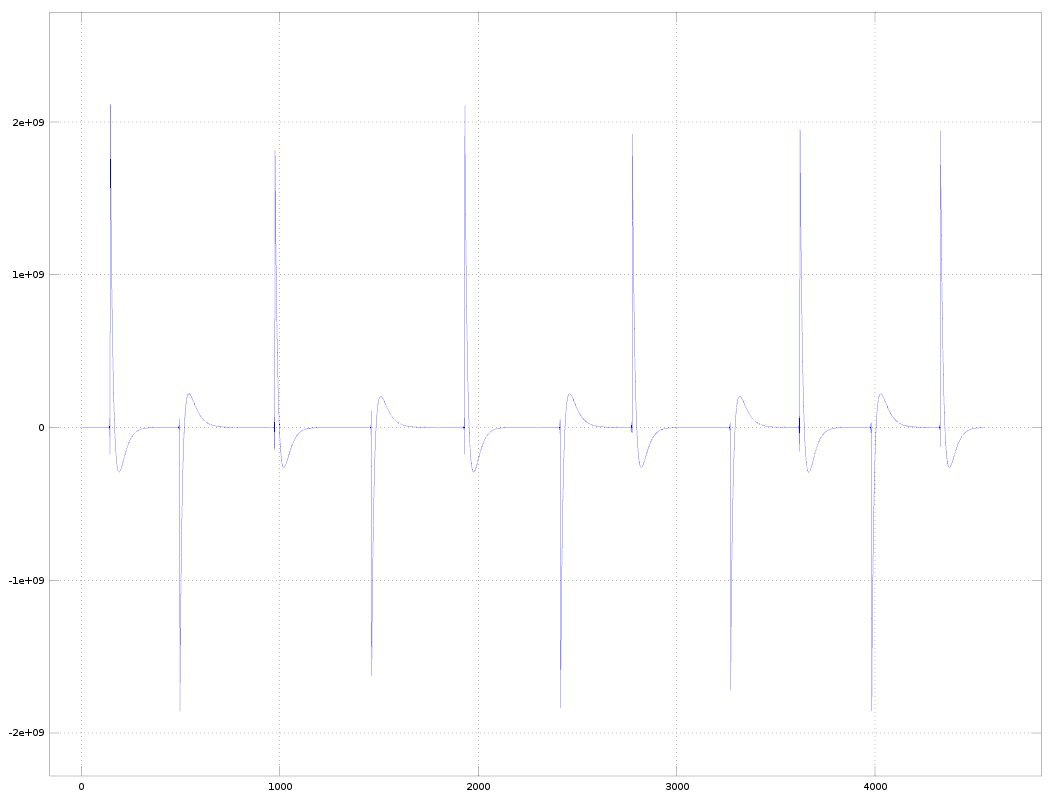
\includegraphics[scale=0.5]{signal-push_buttons.jpg}
  \caption{Поток байтов при нажатии кнопок гарнитуры}
  \label{image:signal}
\end{figure}

На графике \ref{image:signal} мы видим 6 положительных пиков и 5 отрицательных пиков. Положительному пику соответствует нажатие кнопки на гарнитуре. Отрицательному пику соответствует отпускание кнопки гарнитуры.

На листингах \ref{plus_peak} и \ref{minus_peak} приведены примеры считанных байтов.

\begin{lstlisting}[caption={Положительный пик (в шестнадцатиричной системе)},label=plus_peak]
fff5 ffed ffe8 fff8 fff7
ffe2 ff17 009c fff1 ff25 0179 fb90 0912
eded 2fff 7fff 7fff 7fff 7fff 7fff 7fff
7fff 7fff 7fff 7fff 7fff 7fff 7fff 7fff
7fff 7fff 7f9b 7ee7 778c 7188 6bd5 656d
6050 5b76 56de 5183 4d63 49
\end{lstlisting}


\begin{lstlisting}[caption={Отрицательный пик (в шестнадцатиричной системе)},label=minus_peak]
fb6 ffb8 ffb6 ffb0 ffb7
ffc1 ffc5 ffc4 ffa3 ffa3 00b7 fd26 0324
fc9e 00d2 0801 8001 8001 8001 8001 8001
8001 8001 8001 8001 8001 8001 8001 8001
8001 8001 8001 80e0 8151 8870 8e3d 94c1
99f9 9ef7 a3bb a8be ac36 b2b0 b37c bc8c
c638 c039 c2be c6a2 c
\end{lstlisting}

Можно заметить, что нажатию кнопки гарнитуры соответствует несколько раз идущих подряд число $7fff_{16} = 32767_{10}$. А отпусканию кнопки гарнитуры соответствует несколько раз идущих подряд число $8001_{16} = -32768_{10}$.
